% !TEX root = ../main.tex

\chapter{State of the art} \label{chap:state-of-the-art}

\section{Basic notation and definitions} \label{sec:notation}
%% the number of variables
%\todo{bold vectors, capital matrices}
In this thesis, the data are described as input-output pairs, $X \in \mathbb{R}^{n \times d}$ and $Y \in \mathbb{R}^{n \times k}$, respectively.
The $i$-th row of $X$ is a $d$-dimensional data point $\bm{x}_{i}$ belonging to the input space $\mathcal{X}\subseteq\mathds{R}^d$. The corresponding outputs $\bm{y}_{i}$ belong to the output space $\mathcal{Y}$.

The nature of the output space defines the problem as {\sl binary classification} if  $\mathcal{Y} = \{-1,+1\}$, {\sl multi-category classification} if $\mathcal{Y} = \{1,2,\dots,k\}$, {\sl regression} if $\mathcal{Y}\subseteq\mathds{R}$ and {\sl vector-valued regression} if $\mathcal{Y}\subseteq\mathds{R}^k$.

Predictive models are functions $f: \mathcal{X} \rightarrow \mathcal{Y}$.
The number of relevant variables is $d^*$.
In feature selection tasks, the number of selected features is $\tilde d$.

A kernel function acting on the elements of the input space is defined as $\mathcal{K}(\bm{x}_{i},\bm{x}_{j})=\langle \phi(\bm{x}_{i}), \phi(\bm{x}_{j})\rangle$, where $\phi(\bm{x})$ is a {\em feature map} from $\mathds{R}^d \rightarrow \mathds{R}^{d'}$.
Feature learning algorithms project the data into a $p$-dimensional space.
%The number of atoms in Dictionary Learning is $p$.

\section{Machine learning} \label{sec:machine_learning}

The term \textit{machine learning} is becoming an ubiquitous buzzword used in a broad number of contexts spanning from computer science, to behavioral science, to philosophy. Figure~\ref{fig:google_trend_ML} shows a A simple visual inspection of the term popularity trend Google Trends\footnote{\url{https://trends.google.com}}, its popularity is still rising

\begin{figure}
  \centering
    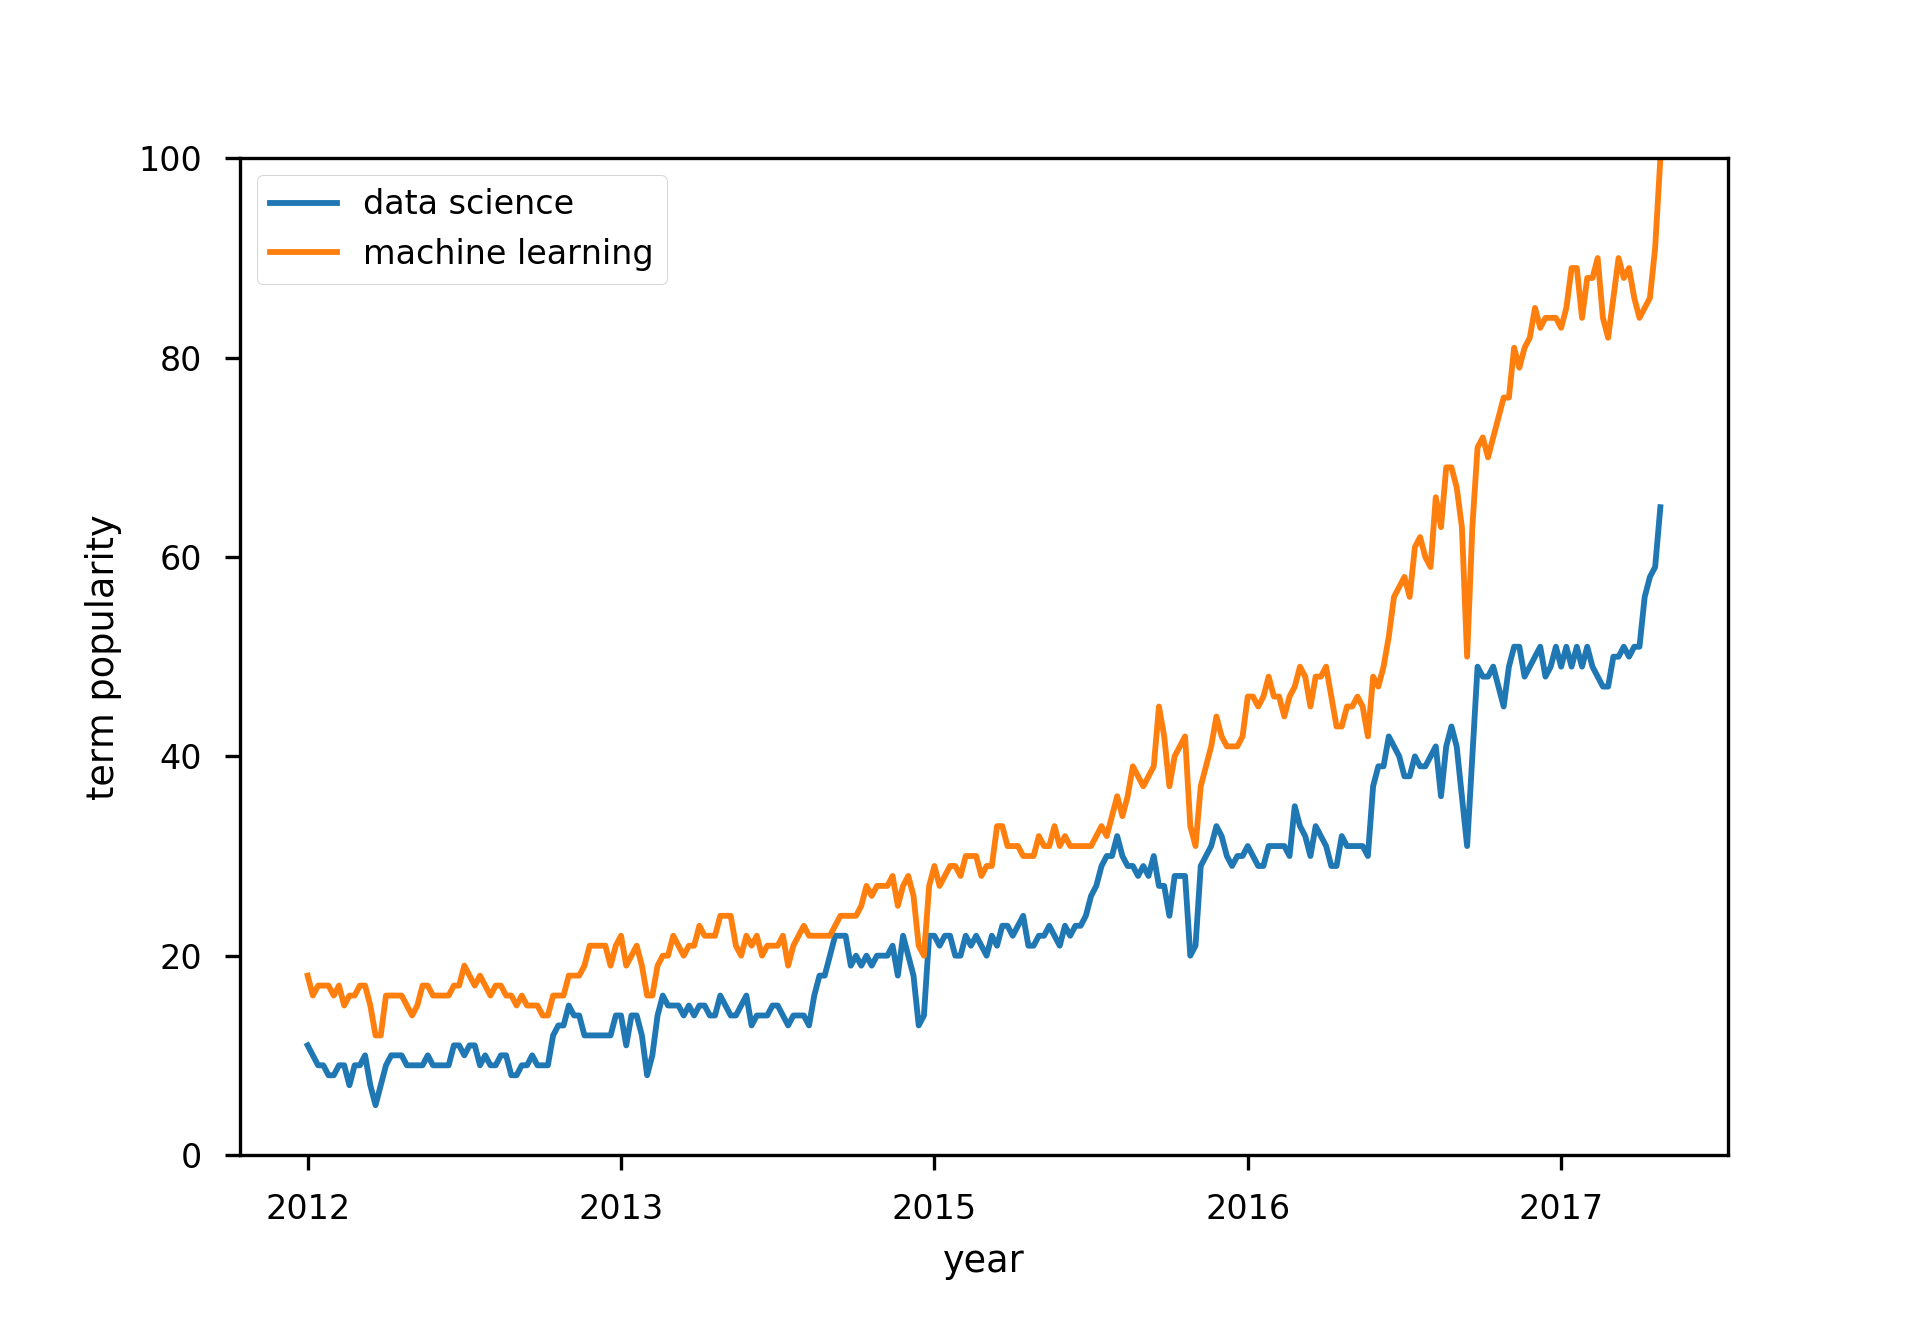
\includegraphics[width=0.8\textwidth]{part1/google_trends_MLDS.png}
  \caption{The web popularity over the last five years of two terms: \textit{data science} and \textit{machine learning} (source: Google Trends).} \label{fig:google_trend_ML}
\end{figure}


% rubare da BIB
In its most classical definition, the aim of modeling is to infer some unknown structure underlying the data. This process can be very hard as many unwanted and concurrent factors may mislead it resulting in a model with poor predictive power.  For instance, the acquisition devices may introduce random fluctuations in the measures or the amount of collected samples may be small with respect to the number of observed variables which, in turn, may not even be representative of the target phenomenon. From a modeling standpoint, every combination of the factors above can be seen as \textit{noise} affecting the data.
Precautions in the model formulation process must be taken in order to achieve solutions that are \textit{robust} to the noise effect.
\todo{maybe we should not introduce noise in such a broad way (see next)}


In the field of machine learning, a common strategy to build predictive models out of noisy data is the \textit{regularization}.
In its broader definition this refers to the process of introducing additional information in order to solve a possibly ill-posed
problem \cite{tikhonov1963solution, evgeniou2000regularization}. The obtained result is a function that fits the training data while having good generalization properties, \ie accurate predictions on previously  \textit{unseen} test data \cite{hastie2009elements}. In machine learning, a model that fits well the training data but performs poorly on new samples is said to be \textit{overfitting} the training set.

  \subsection{Supervised learning} \label{subsec:supervised_learning}
    \subsubsection{Regularization methods}
    \subsubsection{Ensemble methods}
    \subsubsection{Deep learning}


  \subsection{Unsupervised learning} \label{subsec:unsupervised_learning}
    \subsubsection{Manifold learning}
    \subsubsection{Clustering}


  \subsection{Model selection and evalutation} \label{subsec:model_selection}
    \subsubsection{Model selection strategies}
    % cross validation flavours
    \subsubsection{Feature selection stability}
    % stability selection
    \subsubsection{Performance metrics}
    % sup and unsup
    % acc, f1, mcc, ...


\section{Computational requirements and implementations} \label{sec:implementation}
\begin{itemize}
  \item MPI
  \item GPU and accelerators
\end{itemize}
